\section{Data Analysis}\label{Section_dataAnalysis}
In this section, we will deep dive into the data used in our model. Frist, we discuss the available datasets and the relevant columns. Then, we will show some charts with interesting patterns.\\

We have over one million lines of Canada wide monthly claims data, starting in january 2016 until today. We can not use data earlier than 2016, since prior 2016 claims were registered in an older system. This significantly changes the underlying claim distribution and makes prior 2016 data non-representative of future data.\\
The data is divided into databases for each region and line of business. The regions we will cover are Quebec ("QC"), Ontario ("ON") and Alberta ("AB"). The two line of business we cover are physical damage ("PHYSDAM") and liability ("LIPD"). The former consists of collisions and comprehensive coverage (theft, vandalism etc.), while the latter includes all damage caused by the insured to a third party. Note that in Quebec due to regulatory differences there is not separation between the two line of businesses. In Quebec the insurance company covers the loss only for its own insured independent of the responsibility and accountability. We name the single line of business in Quebec "PDPD". We will adjust our model hyper-parameters to each of the regions and lines of business. \\

	\subsection{Data sample}
	The dataset has over 120 columns, so we have to first determine what variables are relevant for us.  The figures  \ref{Fig_sample_1} and  \ref{Fig_sample_2} show and extract for a fictive claim number. The claim number is unique for each claim. Each line represents a month of observation (\texttt{obs\_month}) and is the snapshot of that claim in that specific month. With exception of the variables \texttt{last\_closed\_month}, \texttt{FINAL\_NET\_PAID\_AMT} and \texttt{FINAL\_ALAE\_AMT}, all the information shown is the information we would have for that month of observation, while the three mentioned variables is information we know today (after the observation month). \texttt{sf\_status} is the variable that indicated if the claim is open or closed at the observation month. On figure \ref{Fig_sample_1}, we also have the month of loss (\texttt{MOL}), the reported date (\texttt{CLM\_REPORTED\_DT}) and the month of closure (\texttt{closed\_month}). \texttt{last\_closed\_month} is the month at which the claim closed for the last time, since claims can reopen, this is important information we don’t have when we predict the IBNR.  \texttt{reported\_dev} is the number of months since the claim has been reported, i.e. the age of the claim. \texttt{CATASTROPHE\_IND}, \texttt{TOTAL\_LOSS\_IND}, \texttt{GLASS\_IND}, \texttt{flag\_43} and \texttt{luxury\_ind} are variables we use to classify our data into \texttt{leaf}. We will discuss this in further detail in section \ref{Sect_Methodologie}. 
	
	\begin{figure}[H]
		\begin{center}
			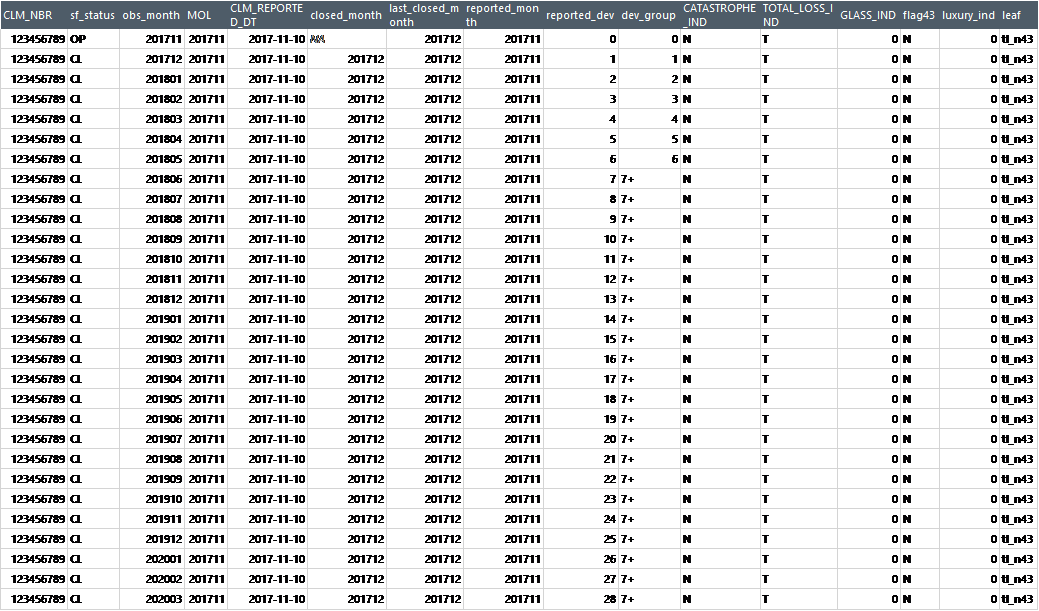
\includegraphics[scale=0.4]{Graphiques/sample_1} 
			\renewcommand{\figurename}{Figure}
			\caption{Sample from database}\label{Fig_sample_1}
		\end{center}
	\end{figure}
	
	In figure \ref{Fig_sample_2}, we have for each month of observation the amounts paid for the loss and ALAE.\\
	\texttt{AUTO\_LTD\_NET\_LOSS\_PAID\_AMT} is the paid amount known at the observation month. Any type of recovery can decrease the paid amount. \texttt{AUTO\_LTD\_LOSS\_RES\_CHG\_AMT} and \texttt{AUTO\_LTD\_LOSS\_RES\_CHG\_AMT} are the case reserve amounts at a given observation month. \texttt{AUTO\_LTD\_LOSS\_INCURRED\_AMT} and \texttt{AUTO\_LTD\_ALAE\_INCURRED\_AMT}, represent the incurred at the given observation month. The variables \texttt{FINAL\_NET\_PAID\_AMT} and \texttt{FINAL\_ALAE\_AMT} are the final amounts we know today, they are also called the ultimate amount for that claim. \texttt{AvgTypicalCarValue} (\texttt{ACV}) is an estimate of the market value of the accident vehicle. \texttt{TotalGAV} (\texttt{GAV}) is the gross appraisal value, which is the garage cost estimate to repair the vehicle. \texttt{IBC\_PRICE} is the initial purchasing price of the vehicle.\\
	\begin{figure}[H]
		\begin{center}
			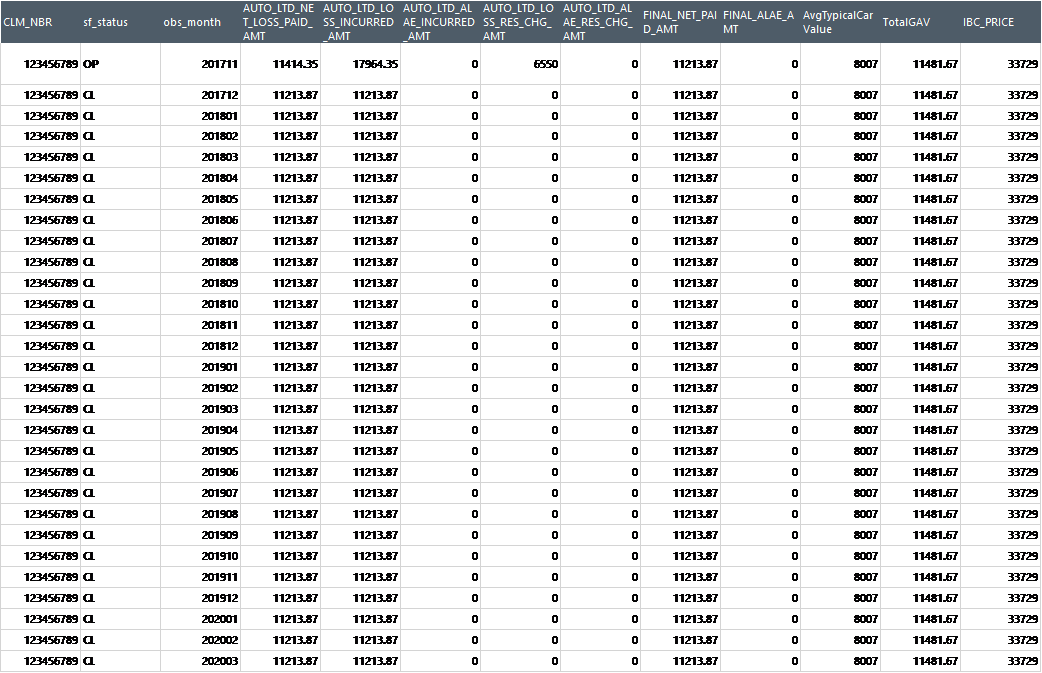
\includegraphics[scale=0.4]{Graphiques/sample_2} 
			\renewcommand{\figurename}{Figure}
			\caption{Severity sample from database}\label{Fig_sample_2}
		\end{center}
	\end{figure}

	Already with this single extract we can get a small understanding of our data. Specifically, we notice that the final paid amount, i.e. the ultimate, is close to \texttt{ACV} and \texttt{GAV} amount. This might indicate that the \texttt{ACV} and \texttt{GAV} are good predictors for our model. Consequently, we want to identify the dependence structure between the ultimate amount and the \texttt{ACV} or \texttt{GAV}. \\
	
	\subsection{Dependence structure}
	\cite{embrechts2001modelling}  show how copulas are used for modelling dependence between random variables. Even thou we do  not plan to model de dependence structure itself, we will use the copula to visualize the dependence. Since we are interested in more than only linear dependence, we will use Kendall’s tau as dependence measure. The definition of Kendall’s tau for a random vector pair $(X,Y)$ is given as
	
	$$ \tau(X,Y) = \Pr( (X - \widetilde{X}) (Y - \widetilde{Y}) > 0 ) - \Pr( (X - \widetilde{X}) (Y - \widetilde{Y}) < 0 )$$
	, where $(\widetilde{X},\widetilde{Y})$ is an independent copy of $(X,Y)$.\\
	
	It is the probability of concordance minus the probability of discordance. Concordance measures how X and Y move in the same direction relative to their independent copy. Discordance measures how X and Y move in opposite direction relative to their independent copy. It also can be interpreted as the correlation coefficient between the quantiles of X and Y, which have a relationship defined by a copula. Kendall’s tau has a value between -1 and 1. -1 indicates perfect negative dependence, also called countermonotonic, while 1 indicates perfect positive dependence, comonotonic. If Kendall’s tau is close to 0, the pairs are likely independent.\\
	A copula is a cumulative distribution function of a multivariate uniformed distribution. The copula of two independent uniform distribution $U_1 \sim U(0,1)$ and $U_2 \sim U(0,1)$, is defined as
	$$C(u_1,u_2) = u_1 \times u_2$$.
	
	A copula can be visualized by plotting pairs of quantiles of the uniform distributions. For the bivariate independent copula, the pairs are evenly distributed on the graph. Kendall’s tau should be close to 0 since it measures the correlation coefficient of these pairs. \\
	Before we can plot the ultimate and the \texttt{ACV/GAV}, we need to find their empirical quantile values between 0 and 1. We rank the values according to their relative size and divide each rank by the total number of observations. In addition, we will only use a sample of 10000 pairs, because we would have to many data points on the graph. We also use one single pair per claim number. Furthermore, we group the data into age since reported date categories. \\
	Starting with Quebec, figures \ref{Fig_copula_qc_rep} to \ref{Fig_copula_qc_tl} shows the copulas for each age grouping. On the x-axis we plot the quantiles of the ultimate amount (paid loss + alae) and on the y-axis we can see the quantiles of the\texttt{GAV}or \texttt{ACV}. We use the\texttt{GAV}for claims with repairable vehicles and the \texttt{ACV} for claims with vehicles that are total loss. On figure XXX we can observe the relationship between the ultimate and \texttt{GAV}. The relationship seems strong especially for younger claims (> 0.7). Note that Kendall’s tau decreases the older the claims become, indicating that older claims become more complex and incurred additional payments or recoveries which do not depend on the damage estimation. Figure XXX demonstrates a weaker dependence between the \texttt{ACV} and the ultimate. However, the dependence is still positive and not negligible. Further, it shows that the \texttt{ACV} might not always be a good estimation of the actual market value. The weaker dependence is therefore only caused by additional fees but also by intrinsic estimation error of the actual market value of the vehicle. 
	
	\begin{figure}[H]
		\begin{center}
			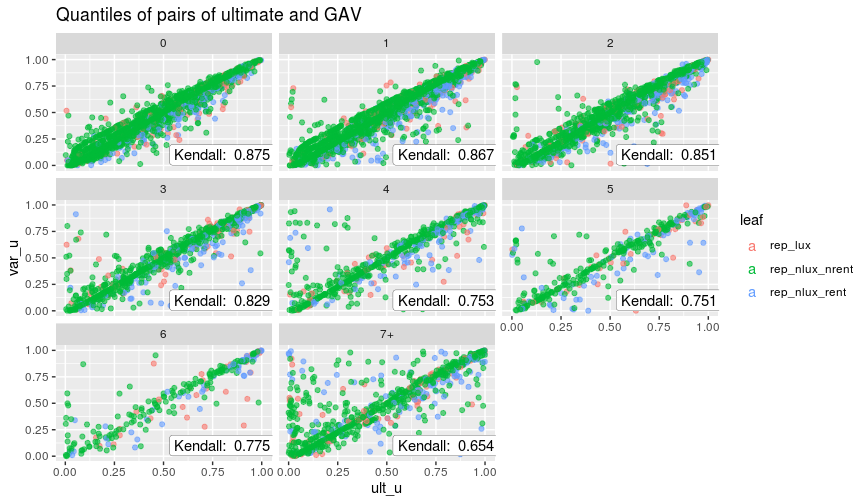
\includegraphics[scale=0.4]{Graphiques/qc_rep} 
			\renewcommand{\figurename}{Figure}
			\caption{Quantiles pairs for Quebec repairable claims. x-axis is the ultimate quantiles and y-axis the \texttt{GAV} quantiles}\label{Fig_copula_qc_rep}
		\end{center}
	\end{figure}

	\begin{figure}[H]
		\begin{center}
			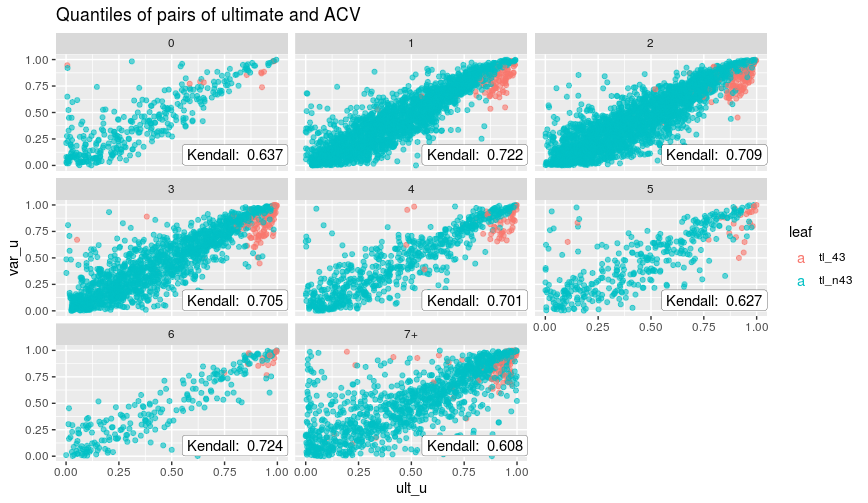
\includegraphics[scale=0.4]{Graphiques/qc_tl} 
			\renewcommand{\figurename}{Figure}
			\caption{Quantiles pairs for Quebec total loss claims. x-axis is the ultimate quantiles and y-axis the \texttt{ACV} quantiles}\label{Fig_copula_qc_tl}
		\end{center}
	\end{figure}

	For Ontario figure\ref{Fig_copula_on_rep} to \ref{Fig_copula_on_tl} show similar pattern than for Quebec. However, since we have two different lines of business PHYSDAM and LIPD, it is interesting to observe the difference in pattern. LIPD tends to be more on the lower half of the diagonal. Third party liabilities seem to incur higher losses than the \texttt{GAV} would suggest and that it incurs more additional fees. 
	
		\begin{figure}[H]
		\begin{center}
			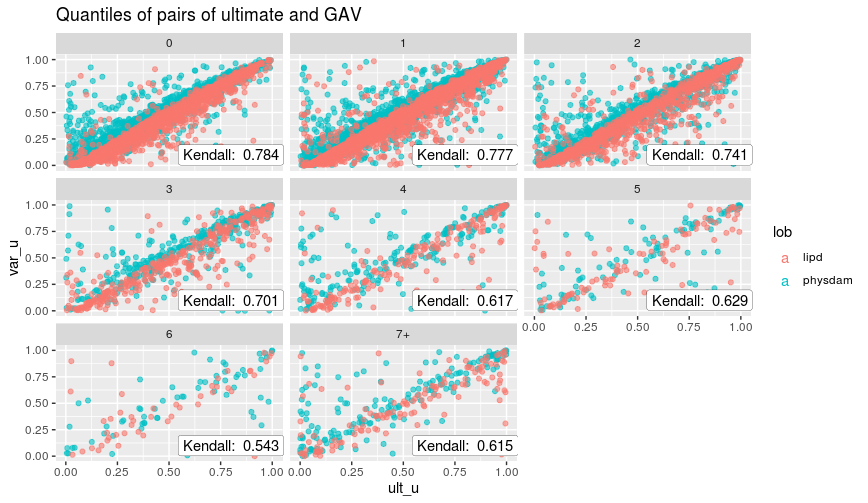
\includegraphics[scale=0.4]{Graphiques/on_rep} 
			\renewcommand{\figurename}{Figure}
			\caption{Quantiles pairs for Ontario repairable claims. x-axis is the ultimate quantiles and y-axis the \texttt{GAV} quantiles}\label{Fig_copula_on_rep}
		\end{center}
	\end{figure}
	
	\begin{figure}[H]
		\begin{center}
			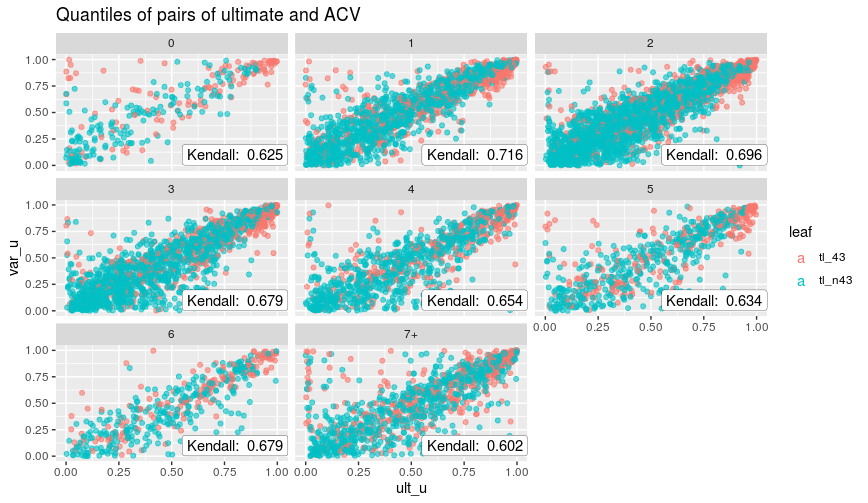
\includegraphics[scale=0.4]{Graphiques/on_tl} 
			\renewcommand{\figurename}{Figure}
			\caption{Quantiles pairs for Ontario total loss claims. x-axis is the ultimate quantiles and y-axis the \texttt{ACV} quantiles}\label{Fig_copula_on_tl}
		\end{center}
	\end{figure}
	
	Alberta shown in figure \ref{Fig_copula_ab_rep} to \ref{Fig_copula_ab_tl} has an interesting patterns. Again, we see weaker dependence for older claims. Albeit, there is a descriptive force which seem to strongly impact the dependence structure and leads to more claims with very low ultimate compared to the \texttt{GAV} or \texttt{ACV}. We identified this disruptive force as subrogation and recoveries. Subrogation is a slow process at which the insurance company can recover paid losses, if the insured was not responsible for the accident. This mean that if Intact paid the entire loss, they might be able to recover a part or the entire loss with a lawsuit. 
	
	\begin{figure}[H]
		\begin{center}
			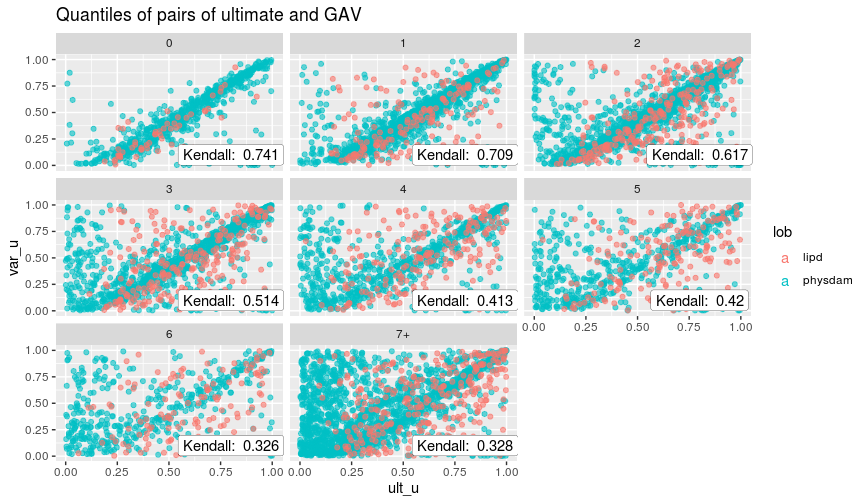
\includegraphics[scale=0.4]{Graphiques/ab_rep} 
			\renewcommand{\figurename}{Figure}
			\caption{Quantiles pairs for Alberta repairable claims. x-axis is the ultimate quantiles and y-axis the \texttt{GAV} quantiles}\label{Fig_copula_ab_rep}
		\end{center}
	\end{figure}
	
	\begin{figure}[H]
		\begin{center}
			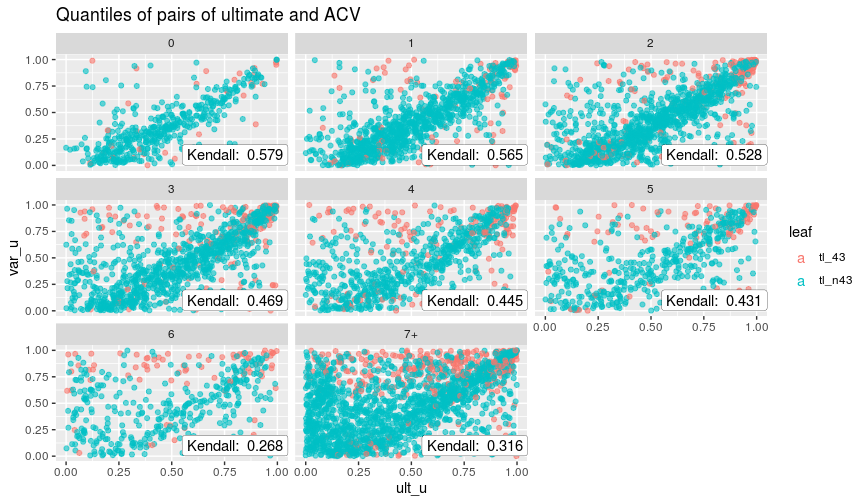
\includegraphics[scale=0.4]{Graphiques/ab_tl} 
			\renewcommand{\figurename}{Figure}
			\caption{Quantiles pairs for Alberta total loss claims. x-axis is the ultimate quantiles and y-axis the \texttt{ACV} quantiles}\label{Fig_copula_ab_tl}
		\end{center}
	\end{figure}

	The data indicates that it can take more than a year until the subrogation process is finished. Consequently, a proportion of claims in Alberta need much longer to fully develop to ultimate which might even fall to 0 or negative. This can be problematic, since we are often unable to predict if the claim falls into the subrogation category or not. We can not filter out these claims, because for a given observation month, we do not know which claims are affected. We can partly mitigate this issue by aggregating the data and using averages. We can expect higher volatility in our model for Alberta. 
	All of these copulas also indicate a slightly stronger dependence for large/extreme values. 
	
	\subsection{Trend analysis}
	
	In our model we do not want to estimate the ultimate on a claim by claim basis, so we will aggregate the data. When aggregating data it is important to verify the trends in data. If we use the \texttt{GAV} and the \texttt{ACV} as a predictor for the ultimate, we should verify that mean growth rates are similar. For each observation month we will calculate the mean ultimate and the mean \texttt{GAV}/\texttt{ACV} of open claims. Then, we will compare their monthly growth rates.  We could also do the same per month of loss, however, we want to analyse the underlying distribution of what we are trying to predict. Our model will predict the ultimate based on observation month data. Each observation month will contain a proportion of claims with different month of loss. While using aggregation per observation month, we have to be aware of possible fluctuations related to different number of claims and different mixtures of month of loss.\\
	When looking at figure \ref{Fig_QC_growth}, we can observe that in Quebec the average ultimate grows faster than the average \texttt{GAV}/ \texttt{ACV}. Using the\texttt{GAV}and \texttt{ACV} as predictor might tend to underestimate the ultimate if we use past averages. 
	
	\begin{figure}[H]
		\begin{center}
			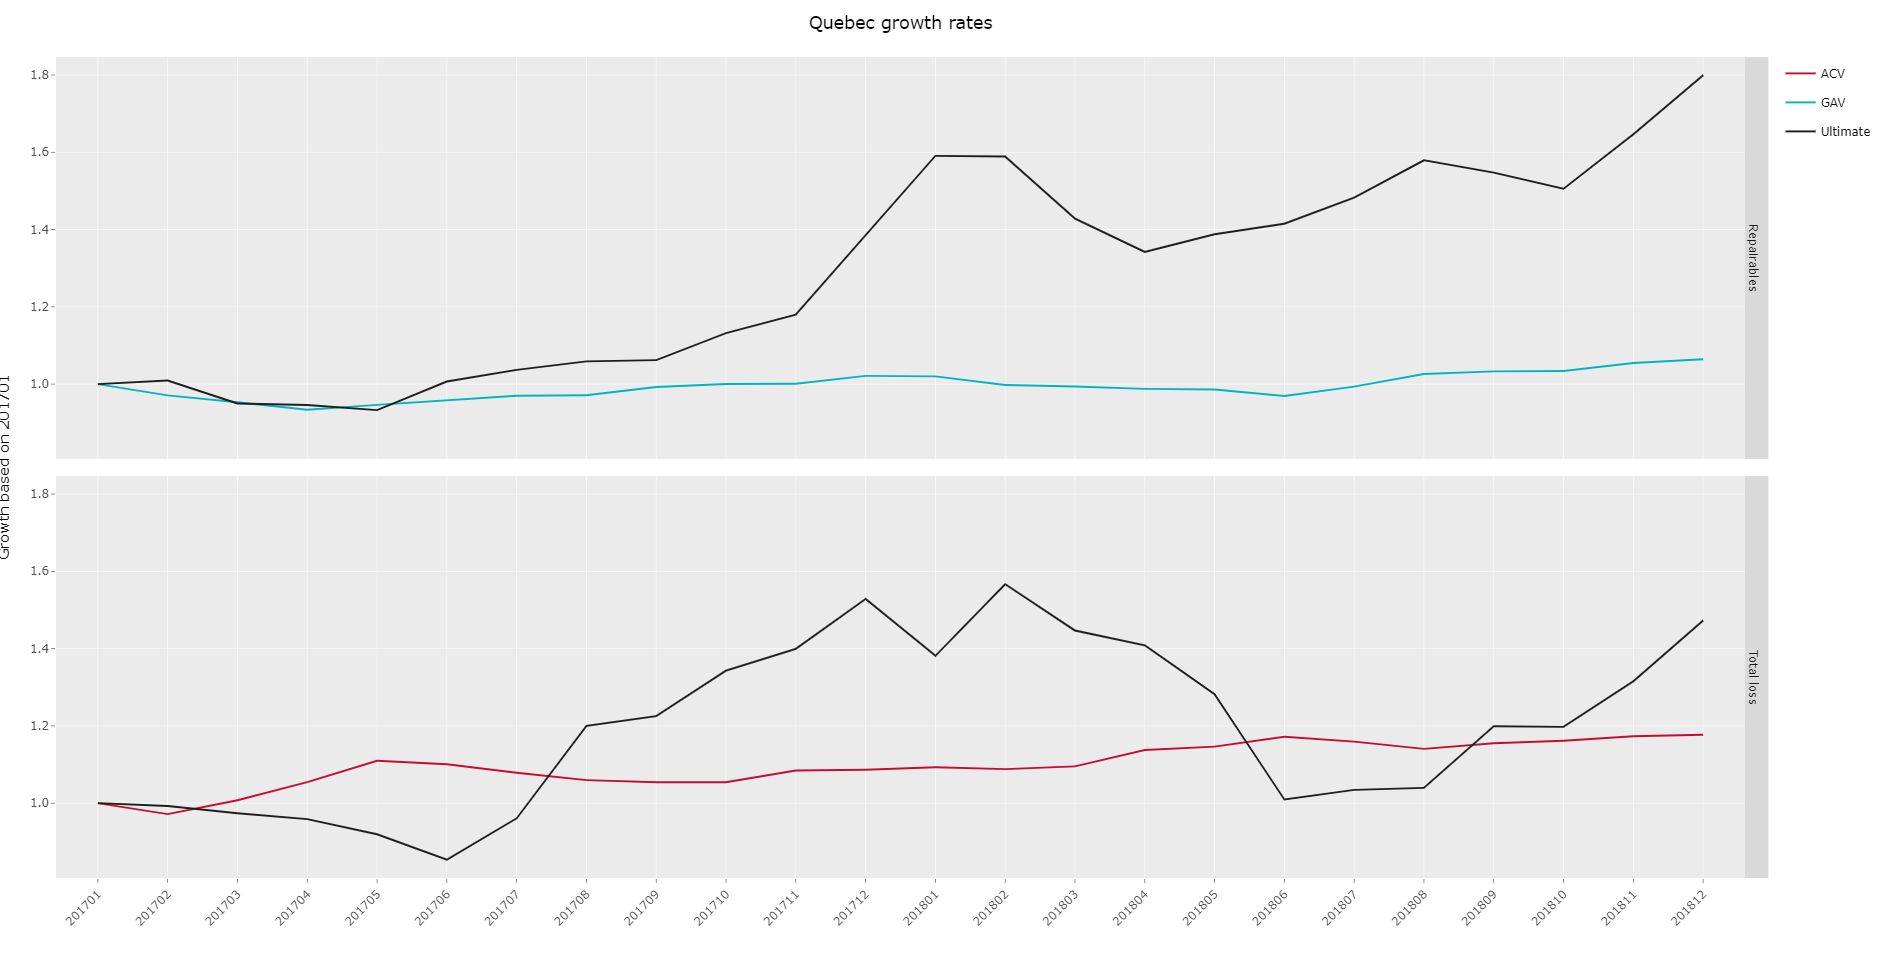
\includegraphics[scale=0.2]{Graphiques/QC_growth} 
			\renewcommand{\figurename}{Figure}
			\caption{Quebec ultimate and \texttt{GAV/ACV} growth relative to January 2017 (= 1)}\label{Fig_QC_growth}
		\end{center}
	\end{figure}

	In Ontario figure \ref{Fig_ON_growth}, the opposite seems to happen for total loss claims but not for repairable. Thus, we might tend to overestimate total loss claims ultimate.
	\begin{figure}[H]
		\begin{center}
			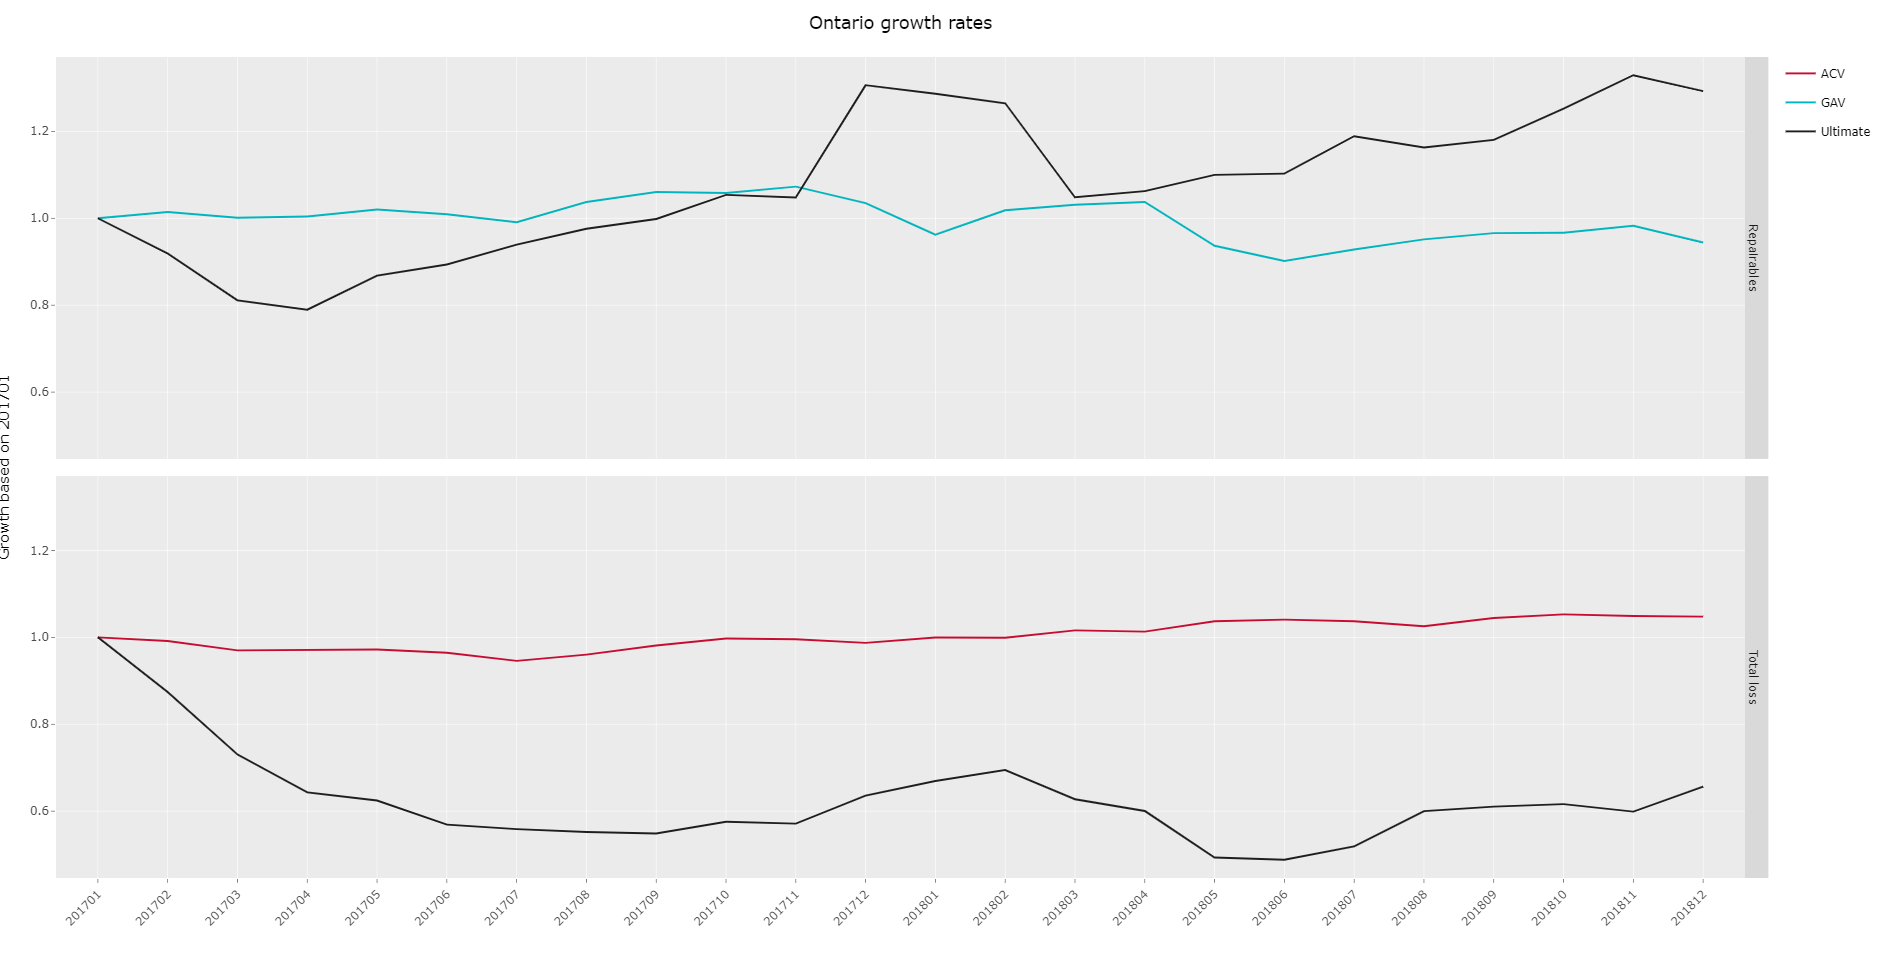
\includegraphics[scale=0.2]{Graphiques/ON_growth} 
			\renewcommand{\figurename}{Figure}
			\caption{Ontario ultimate and \texttt{GAV/ACV} growth relative to January 2017 (= 1)}\label{Fig_ON_growth}
		\end{center}
	\end{figure}
	On figure \ref{Fig_AB_growth}, Alberta has a similar but reversed pattern. Total loss claims ultimate growth fluctuates around the 1 value. While for repairables, growth rates for the ultimate are lower than for the \texttt{GAV}.  
	\begin{figure}[H]
		\begin{center}
			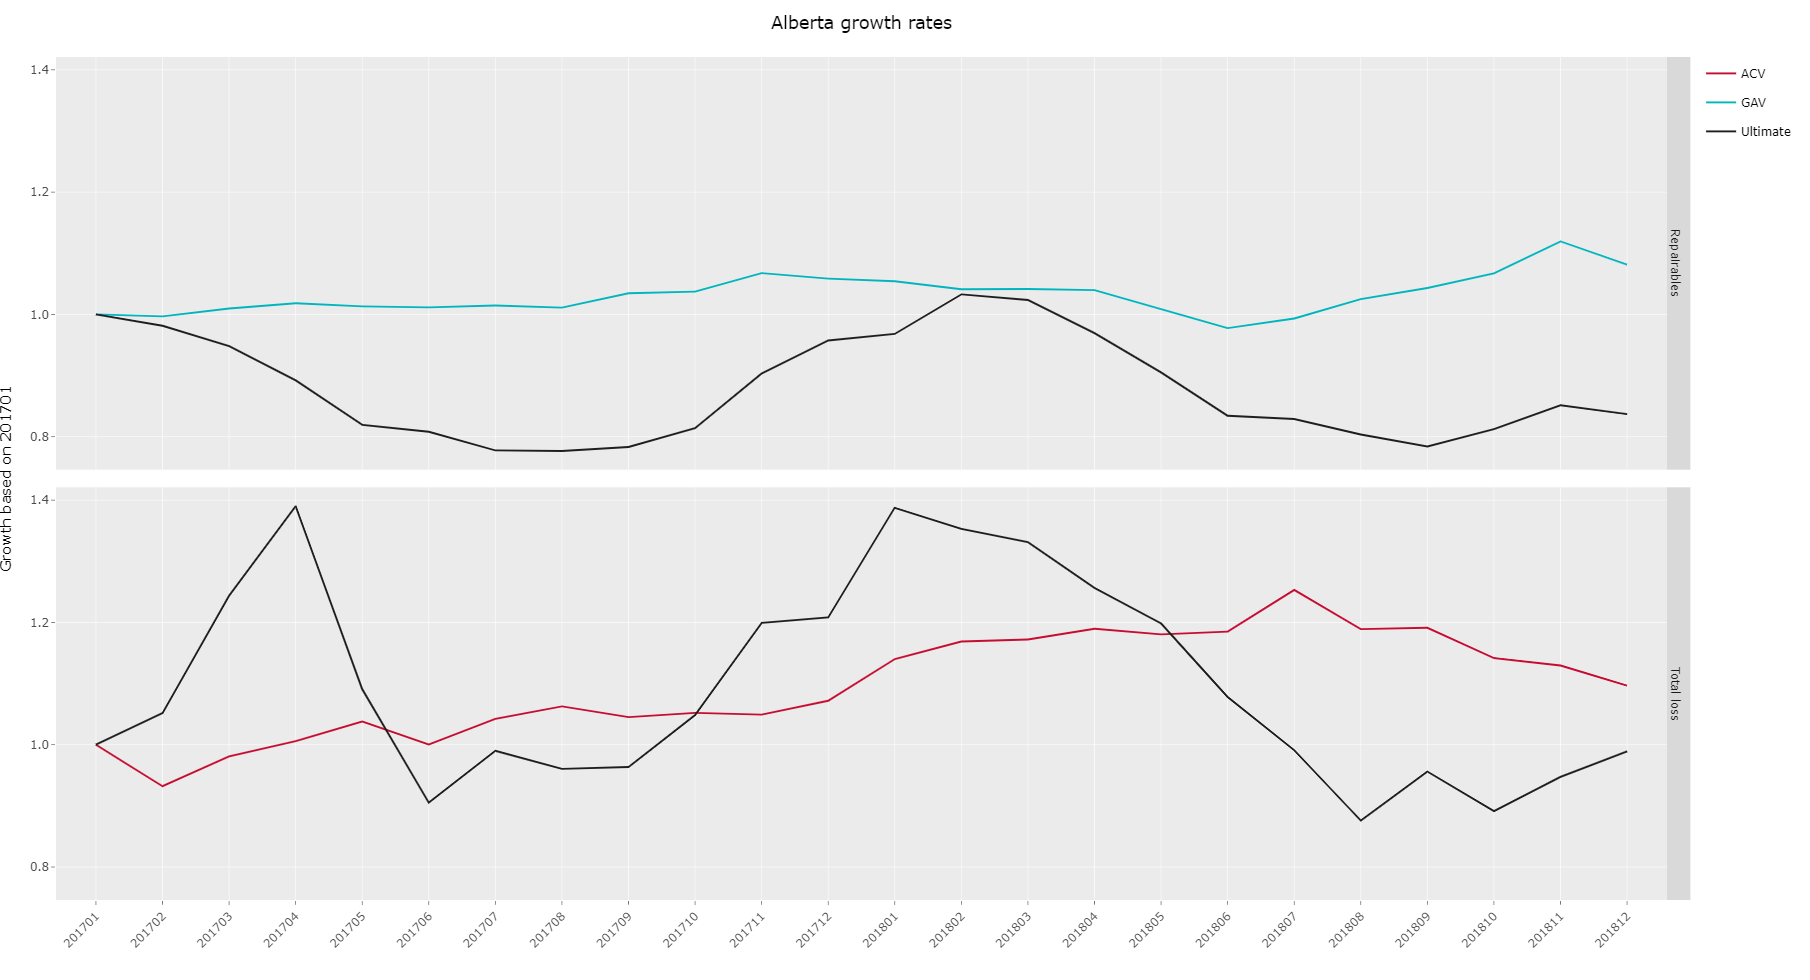
\includegraphics[scale=0.2]{Graphiques/AB_growth} 
			\renewcommand{\figurename}{Figure}
			\caption{Alberta ultimate and \texttt{GAV/ACV} growth relative to January 2017 (= 1)}\label{Fig_AB_growth}
		\end{center}
	\end{figure}

	Furthermore, the \texttt{GAV} and \texttt{ACV} might not capture the additional costs related to the claim. The ultimate allocated loss adjustment expense (ALAE) is often unrelated to the \texttt{GAV} or \texttt{ACV}. A larger proportion of ALAE can cause greater estimation error. Figure \ref{Fig_QC_ALAE_loss} shows the ALAE to loss ratio for Quebec. The average is around 0.0125. In Ontario, seen in figure \ref{Fig_ON_ALAE_loss}, the ALAE to loss ratio is similar to the Quebec, although after December 2017 there is clearly a spike which might cause prediction errors. Alberta in figure \ref{Fig_AB_ALAE_loss} show again a different pattern than the other 2 regions. While most ratios are lower than in Quebec and Ontario, le non-luxury  non-rental repairable vehicles show proportionally larger ratios. 
	
	\begin{figure}[H]
		\begin{center}
			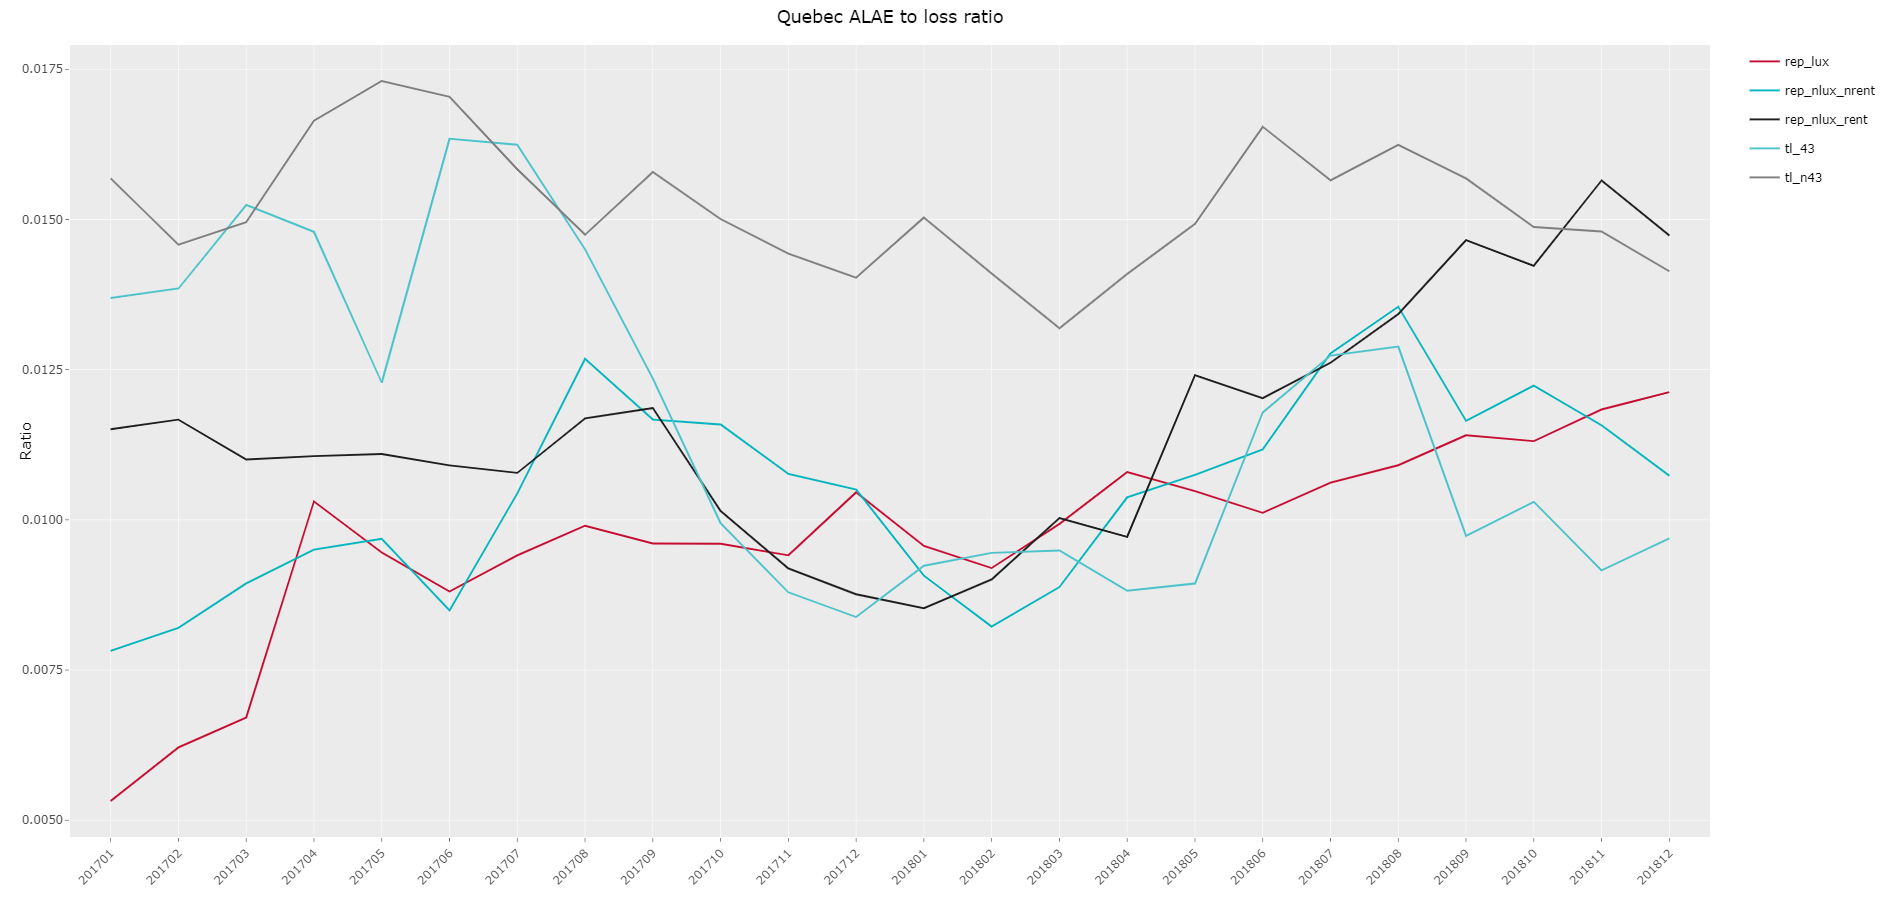
\includegraphics[scale=0.2]{Graphiques/QC_ALAE_loss} 
			\renewcommand{\figurename}{Figure}
			\caption{Quebec ALAE to loss ratio per \texttt{leaf}}\label{Fig_QC_ALAE_loss}
		\end{center}
	\end{figure}

	\begin{figure}[H]
		\begin{center}
				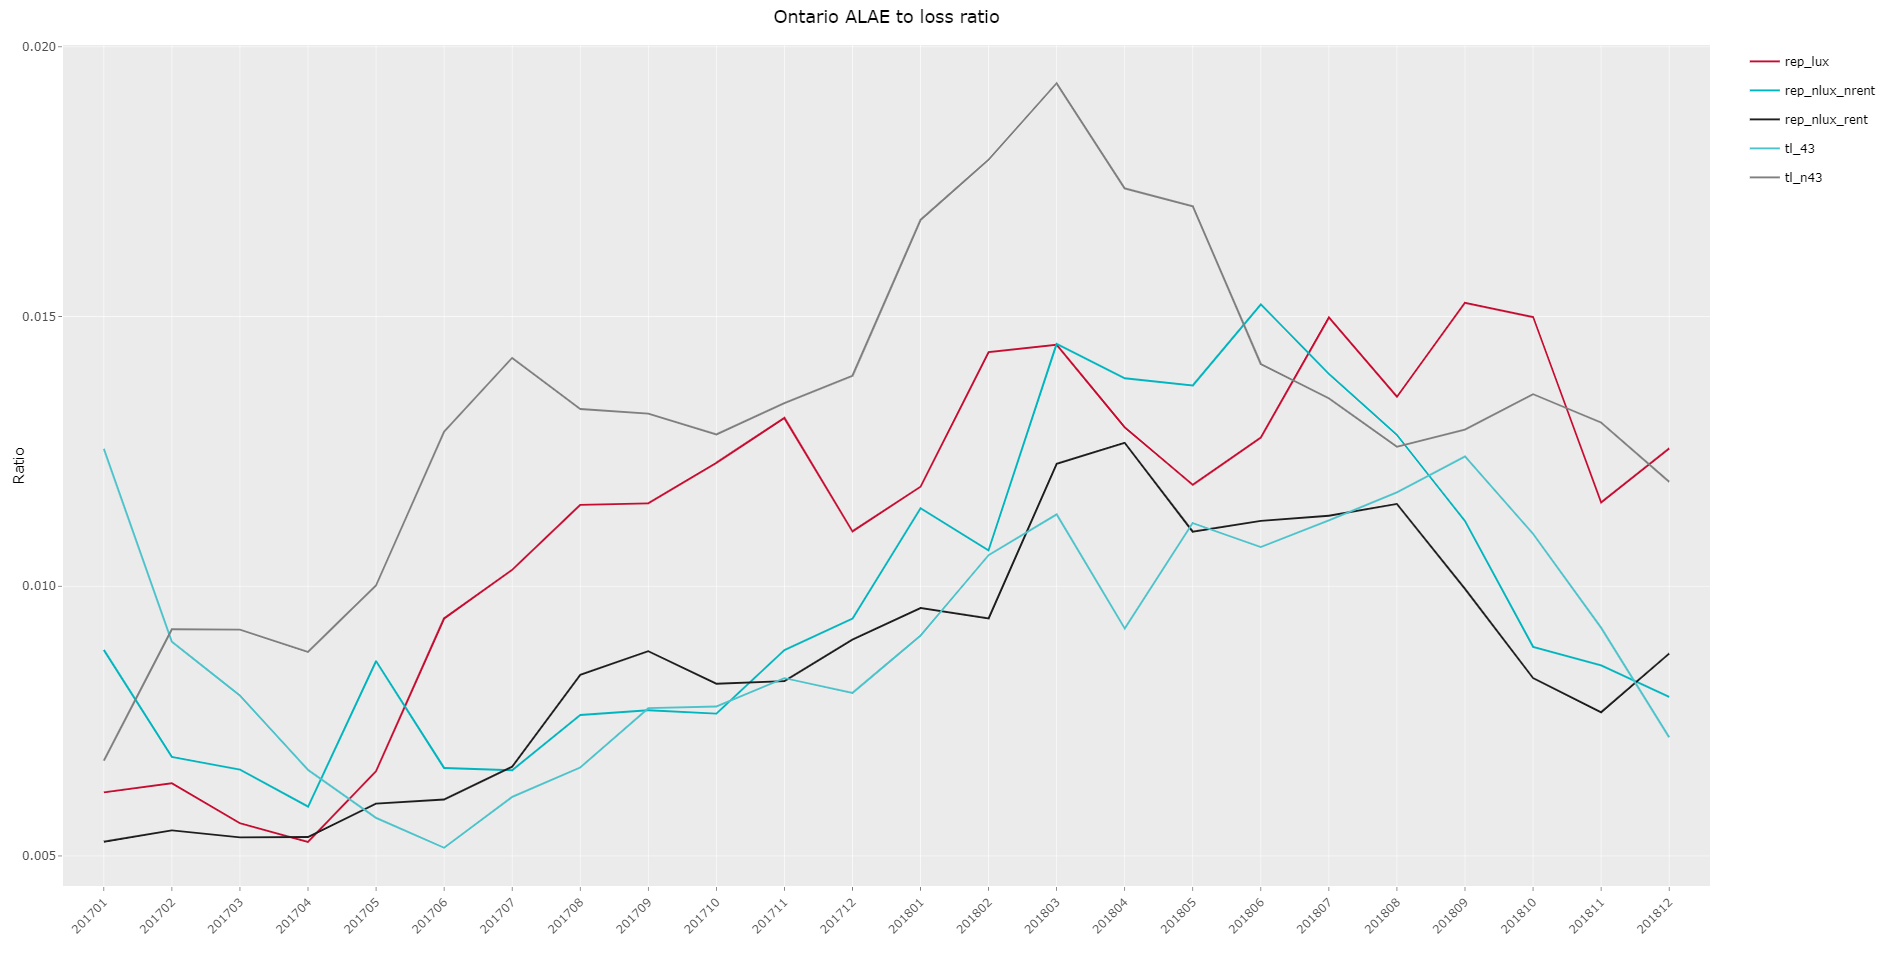
\includegraphics[scale=0.2]{Graphiques/ON_ALAE_loss} 
			\renewcommand{\figurename}{Figure}
			\caption{Ontario ALAE to loss ratio per \texttt{leaf}}\label{Fig_ON_ALAE_loss}
		\end{center}
	\end{figure}
	
	\begin{figure}[H]
		\begin{center}
				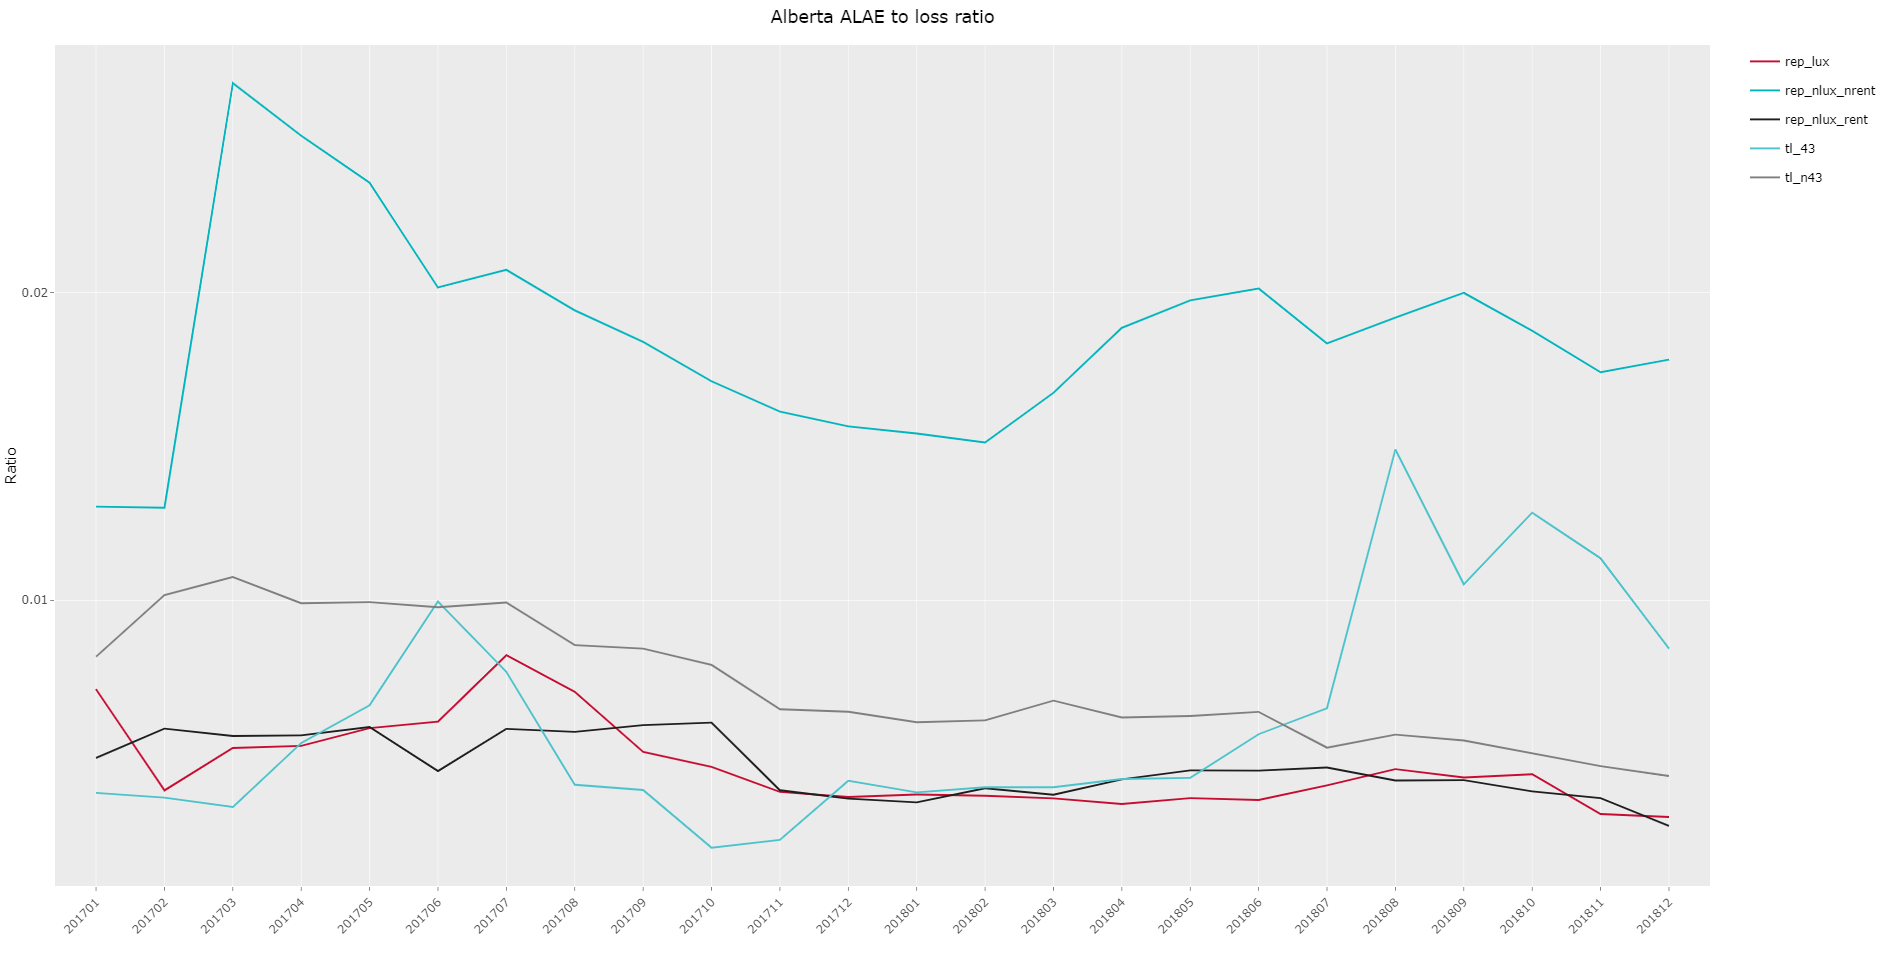
\includegraphics[scale=0.2]{Graphiques/AB_ALAE_loss} 
			\renewcommand{\figurename}{Figure}
			\caption{Alberta ALAE to loss ratio per \texttt{leaf}}\label{Fig_AB_ALAE_loss}
		\end{center}
	\end{figure}
	In order to better understand the impact of recovery on our data, figures \ref{Fig_QC_recovery_loss} to \ref{Fig_AB_recovery_loss} shows the recovery to ultimate ratio for all 3 regions. Quebec and Ontario both have a ratio below 0.17, while Alberta has ratios between 1 and 0.3. The discrepancy is very significant and has to be considered in our model.
		\begin{figure}[H]
		\begin{center}
			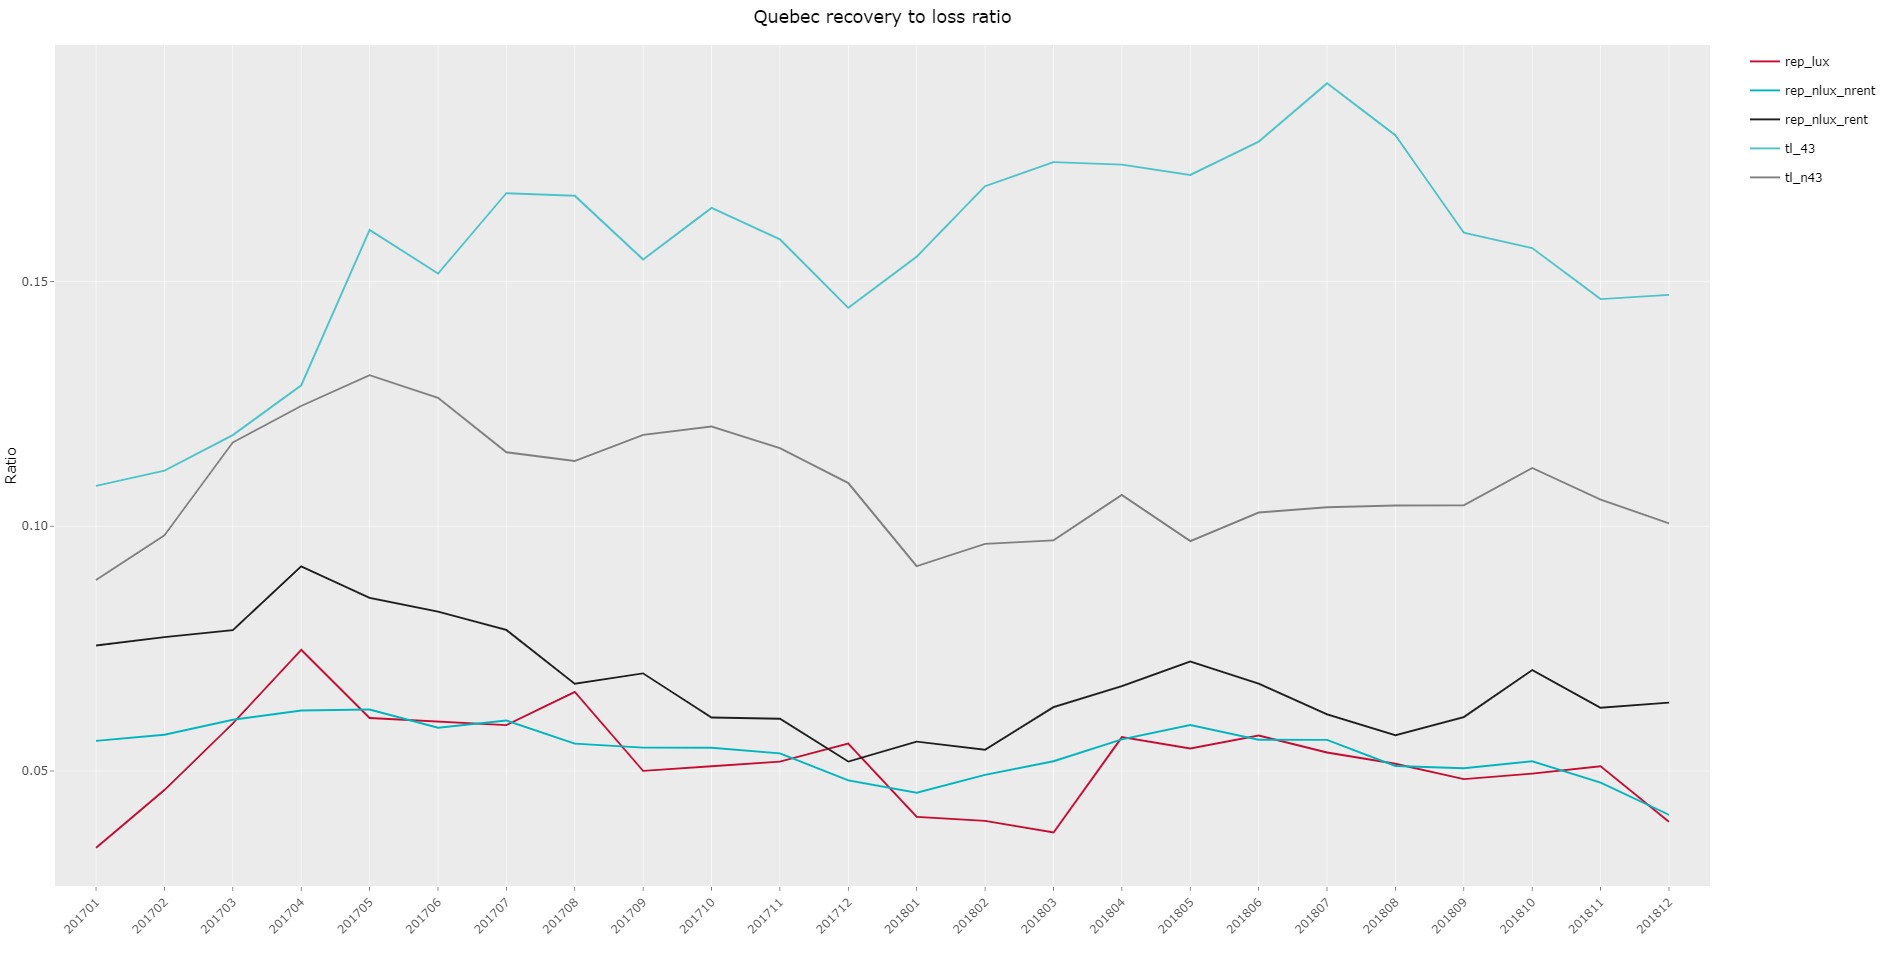
\includegraphics[scale=0.2]{Graphiques/QC_recovery_loss} 
			\renewcommand{\figurename}{Figure}
			\caption{Quebec recovery to loss ratio per \texttt{leaf}}\label{Fig_QC_recovery_loss}
		\end{center}
	\end{figure}
	
	\begin{figure}[H]
		\begin{center}
			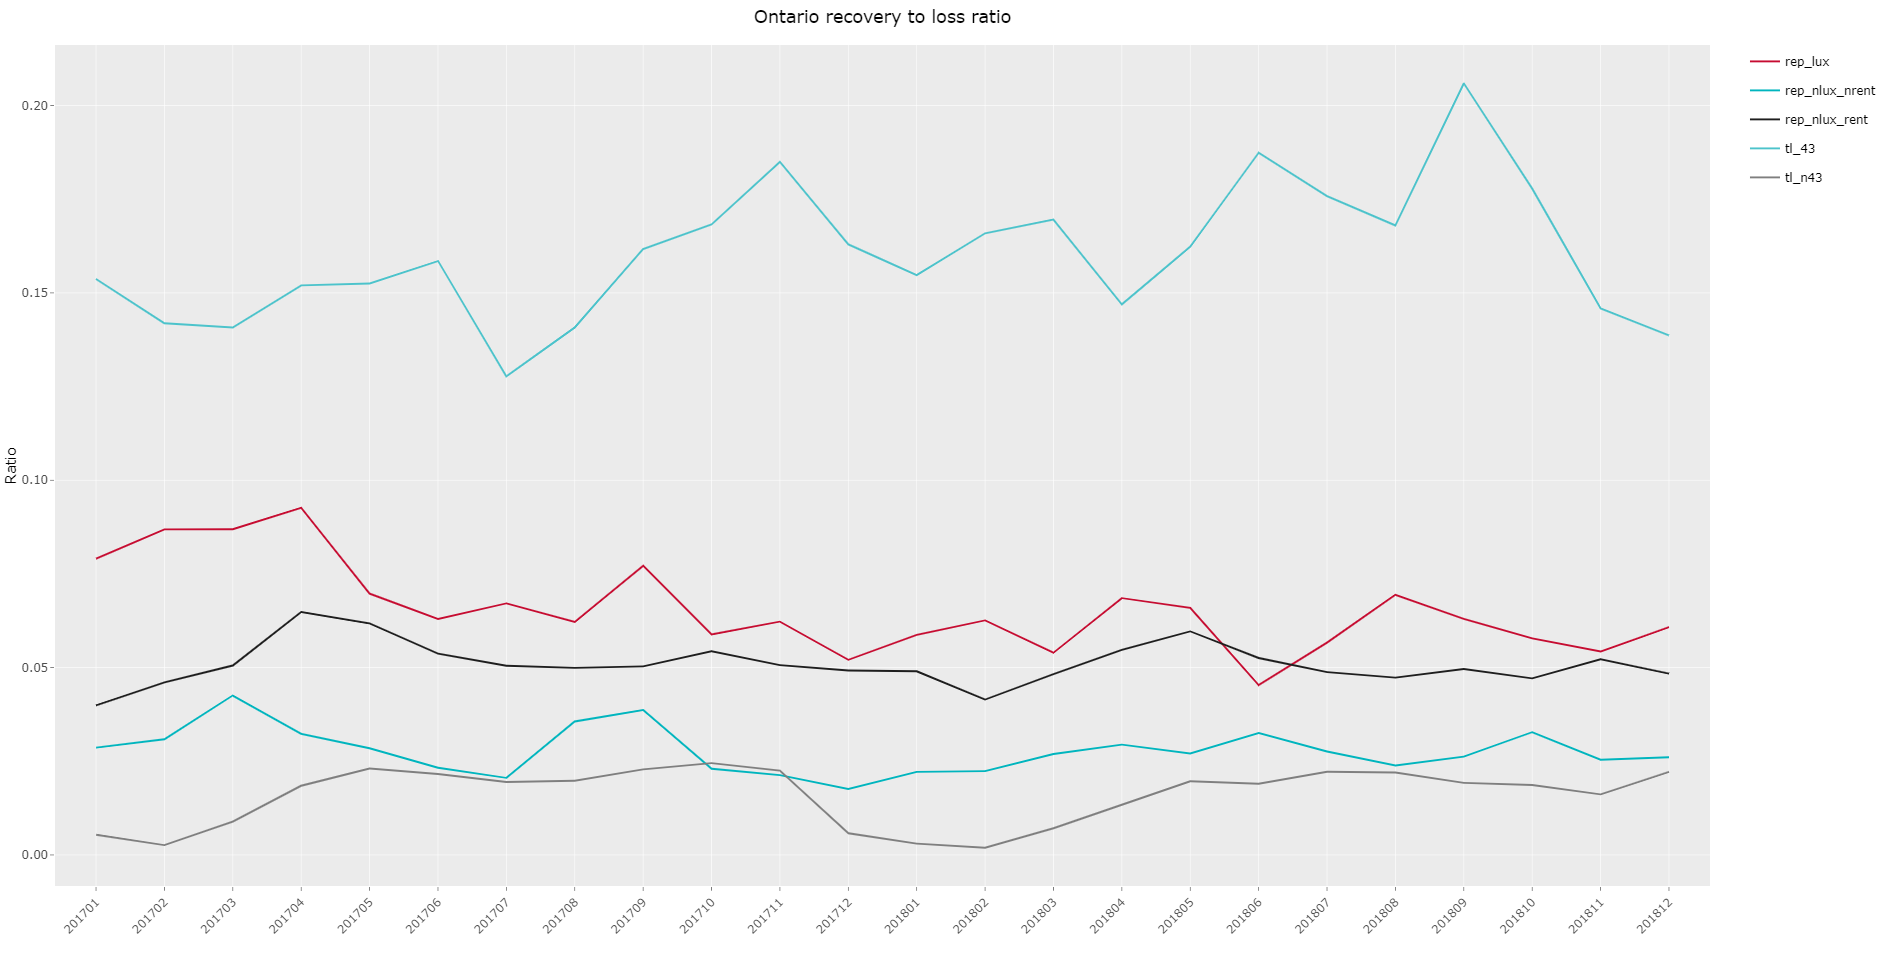
\includegraphics[scale=0.2]{Graphiques/ON_recovery_loss} 
			\renewcommand{\figurename}{Figure}
			\caption{Ontario recovery to loss ratio per \texttt{leaf}}\label{Fig_ON_recovery_loss}
		\end{center}
	\end{figure}
	
	\begin{figure}[H]
		\begin{center}
			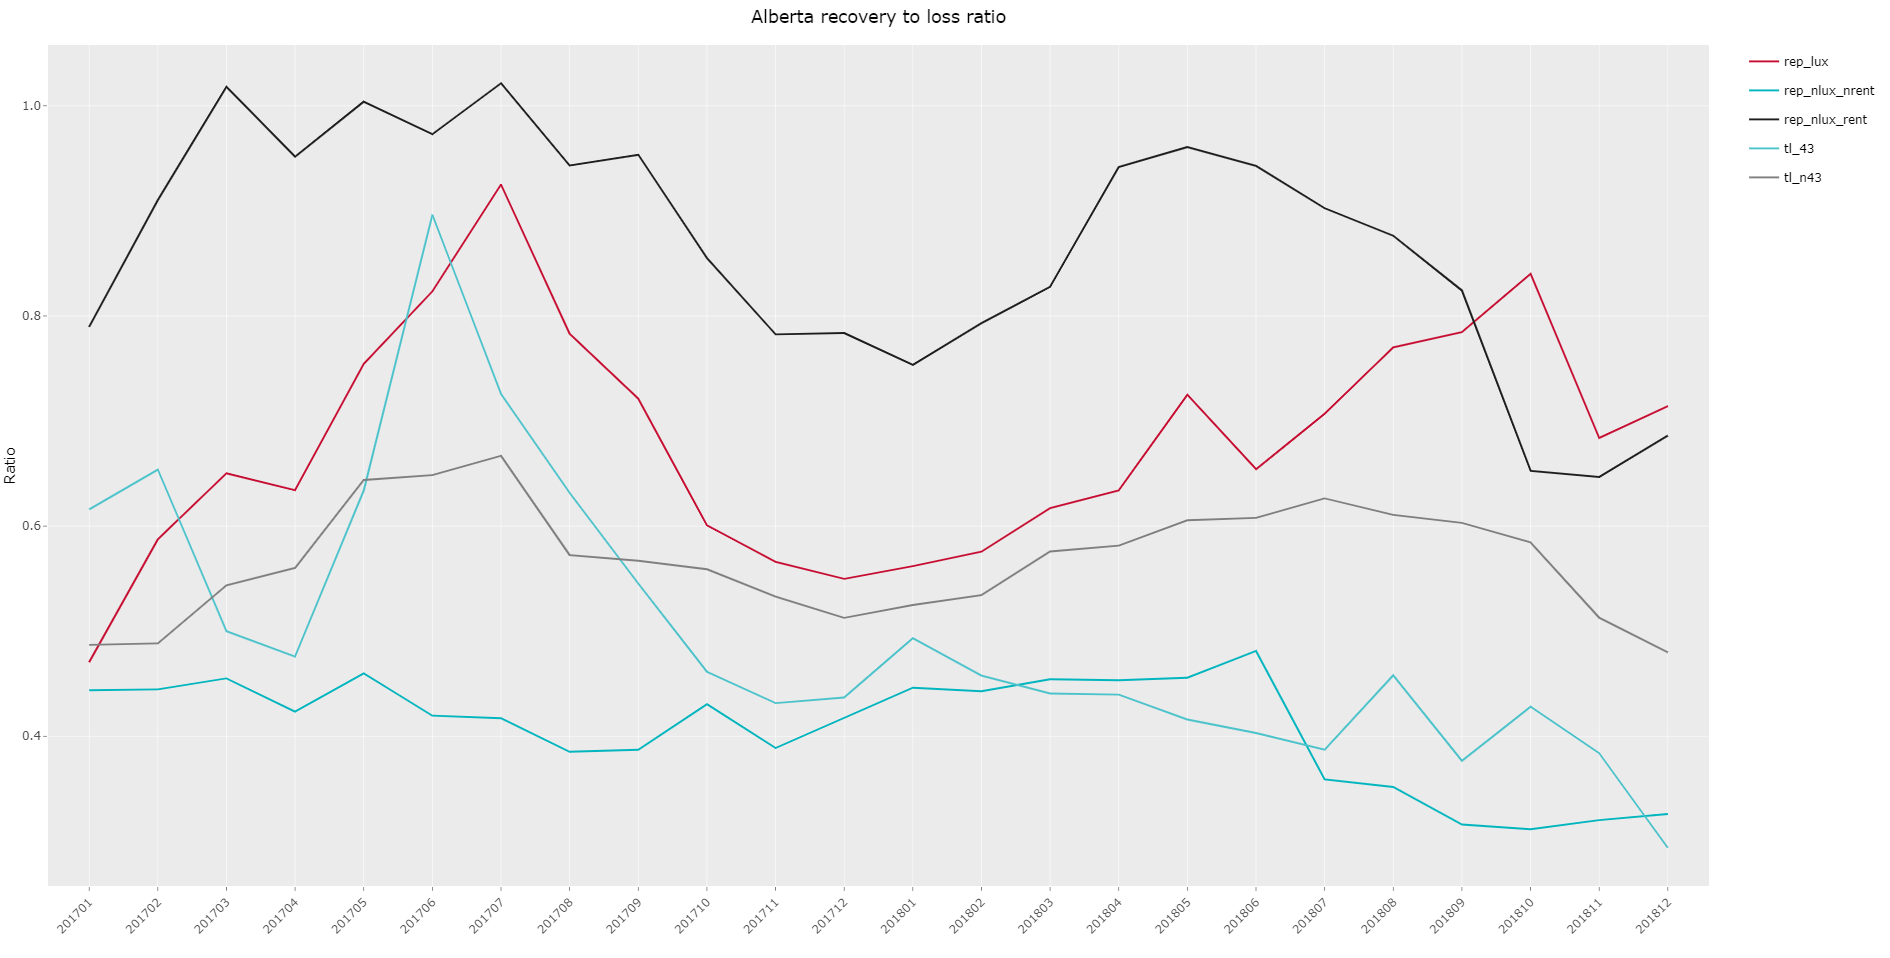
\includegraphics[scale=0.2]{Graphiques/AB_recovery_loss} 
			\renewcommand{\figurename}{Figure}
			\caption{Alberta recovery to loss ratio per \texttt{leaf}}\label{Fig_AB_recovery_loss}
		\end{center}
	\end{figure}
	
	Now that we have a better understanding of our data, we will discuss the model structure and methodology.
	
	 